\documentclass{article}

\usepackage{graphicx} % more modern
\usepackage{subfigure} 
\usepackage{amssymb}
\usepackage{amsmath}
\usepackage{amsthm}


% For citations
\usepackage{natbib}

% For algorithms
\usepackage{comment}
\usepackage{algorithm}
\usepackage{algorithmic}

\usepackage{hyperref}

\allowdisplaybreaks

\newcommand{\theHalgorithm}{\arabic{algorithm}}

\newtheorem{theorem}{Theorem}[section]
\newtheorem{lemma}[theorem]{Lemma}
\newtheorem{conjecture}[theorem]{Conjecture}
\newtheorem{proposition}[theorem]{Proposition}
\newtheorem{definition}[theorem]{Definition}
\newtheorem{corollary}[theorem]{Corollary}

\usepackage[accepted]{icml2012}  % XXX : just set temporarly to print out authors corretly.


\begin{document} 

\icmltitle{Mathematical formulas discovery}

\icmlauthor{Wojciech Zaremba}{zaremba@cs.nyu.edu}
\icmlauthor{Karol Kurach}{kkurach@google.com}
\icmlauthor{Yoram Singer}{singer@google.com}
\icmlauthor{Rob Fergus}{fergus@cs.nyu.edu}


\icmlkeywords{machine learning, optimization, automatic theorem
@inproceedings{Kriz12,
author = {Krizhevsky, A. and Sutskever, I. and Hinton, G.E.},
title = {ImageNet Classification with Deep Convolutional Neural Networks},
booktitle = {NIPS},
year = {2012}
}
 proving, RBM, NP, Boltzmann machine}

\vskip 0.3in


\begin{abstract} 
abstract 
\end{abstract} 


\section{Introduction} \label{introduction} 
Progress in some branches of
mathematics might be restricted by size of symbolic derivations that human can
handle.  Mathematicians can deal with expressions having up to some small
number of variables having different purposes in equations. However, there
might exists very handy relations between expressions having hundreds or
thousands of variables. We will show how task of finding equivalent
mathematical expressions can be automated. Our focus is on finding equivalent
mathematical formulas, which are faster to compute than the original one. Where
faster can be defined as (1) number of operations, or (2) computational time
for any particular computational hardware.


We develop deterministic framework, which discovers relations between
multi-variable polynomial expressions. CLARIFY RESTRICTED TO POLYNOMIALS.  First, we construct grammars of
admissible operations together with cost of every operation. Through linear
combination of grammar elements, we find MINIMUM COST? solution to desired expressions that
we want to compute. Finally, we show that this computation solution can be
further speed up by use of standard techniques of optimization in compiler
domain. We show power of presented approach by deriving close form, linear time
solutions SURELY ACCURATE APPROXIMATIONS to compute partition function like expressions for RBMs. Presented
close form solutions oppose widespread believe that hardness of partition
function computation is in its exponential number of elements.


Finally, we look on set of generated rules as on small axiomatic system.
Presented algorithm is deterministic, finite time proof in this system.
We are excited about using machine learning for automatic reasoning, and
this subset of mathematics seem to be perfect fit for testing automatic reasoning systems.
Usually, axiomatic systems like number theory, set theory, or topology have very small
number of axioms, but their application to terms might be complex. Proofs
for such systems are difficult to represent in software, and there is no
baseline algorithms which could brute force proof by iterating over all of them in reasonable finite time.
Where in the contrary, presented here axiomatic system has very simple representation
in software, and this paper presents brute force algorithm to find
proofs. WITHIN POLYNOMIALS ONLY?
Surprisingly, even brute force algorithm is able to find new more efficient,
computational expressions for expressions that we use.

ANOTHER POTENTIAL APPROACH TO COMPUTING PARTITION FUNCTION. 
ALSO GENERIC APPROACH FOR COMPUTATIN.

DISCUSSION OF LEARNING HERE. MOVE TO PROBABILISTIC GRAMMARS AND LEARN
FROM LOWER POWERS WHAT COMBINATIONS OF RULES ARE LIKELY TO WORK. 

MAYBE HAVE SIMPLE EXAMPLE HERE.


\section{Related work} \label{relatedwork}

compilers, computer vision grammars, nlp grammars. Finding rules in physics.

\section{Admissible computation as a grammars}\label{sec:grammars}

We consider grammar on tuples : (expression, computation, computational time).
We focus attention on expressions, which are matrices of polynomials. We denote
matrix of size $n \times m$ of $k$-th degree polynomials by $\mathcal{P}^{n
\times m}_k$.  The final goal is to find tuple for a given expression having
a shortest computational time. Where computational time is any measure of
complexity, which we care about. For instance, for theoretical computer science
purposes it might be number of operations, or computation complexity. However,
from perspective of engineering, it might be computation time on specific GPU
model. 


Let's ground our approach in an example. We assume that we are interest in
finding algorithm with smallest operation complexity, and computation platform
is a Matlab.  We consider following set of operations on matrices : 

\begin{align*}
&\text{{\bf Element wise multiplication}}\\
&(a \in \mathcal{P}^{n \times m}_\alpha, A, t_1), (b \in \mathcal{P}^{n \times m}_\beta, B, t_2) \rightarrow \\ 
&(c \in \mathcal{P}^{n \times m}_{\alpha + \beta}, A .* B, O(t_1 + t_2 + nm)) \\
&c_{i,j} = a_{i,j}b_{i, j} \text{ for } i \in \{1, \dots, n\}, j \in \{1, \dots, m\} \\
&\text{{\bf Matrix multiplication}}\\
&(a \in \mathcal{P}^{n \times m}_\alpha, A, t_1), (b \in \mathcal{P}^{m \times k}_\beta, B, t_2) \rightarrow \\ 
&(c \in \mathcal{P}^{n \times k}_{\alpha + \beta}, A * B, O(t_1 + t_2 + nmk)) \\
&c_{i,k} = \sum_{k = 1}^K a_{i,k}b_{k, j} \text{ for } i \in \{1, \dots, n\}, j \in \{1, \dots, m\} \\
%%% WOJCIECH TO CHECK
&\text{{\bf Columns marginalization}}\\
&(a \in \mathcal{P}^{n \times m}_\alpha, A, t_1) \rightarrow \\ 
&(c \in \mathcal{P}^{n \times 1}_\alpha, sum(A, 2), O(t_1 + nm)) \\
&c_{i, 1} = \sum_{j = 1}^m a_{i, j} \text{ for } i \in \{1, \dots, n\}\\
&\text{{\bf Rows marginalization}}\\
&(a \in \mathcal{P}^{n \times m}_\alpha, A, t_1) \rightarrow \\ 
&(c \in \mathcal{P}^{1 \times m}_\alpha, sum(A, 1), O(t_1 + nm)) \\
&c_{1, j} = \sum_{i = 1}^m a_{i, j} \text{ for } j \in \{1, \dots, m\}\\
&\text{{\bf Columns repetition}}\\
&(a \in \mathcal{P}^{n \times 1}_\alpha, A, t_1) \rightarrow \\ 
&(c \in \mathcal{P}^{n \times m}_\alpha, repmat(A, 1, m), O(t_1 + nm)) \\
&c_{i, j} = a_{i, 1} \text{ for } i \in \{1, \dots, n\}\\
&\text{{\bf Rows repetition}}\\
&(a \in \mathcal{P}^{1 \times m}_\alpha, A, t_1) \rightarrow \\ 
&(c \in \mathcal{P}^{n \times m}_\alpha, repmat(A, n, 1), O(t_1 + nm)) \\
&c_{i, j} = a_{1, j} \text{ for } j \in \{1, \dots, m\}\\
&\text{{\bf Entry repetition}}\\
&(a \in \mathcal{P}^{1 \times 1}_\alpha, A, t_1) \rightarrow \\ 
&(c \in \mathcal{P}^{n \times m}_\alpha, repmat(A, n, m), O(t_1 + nm)) \\
&c_{i, j} = a_{1, 1} \text{ for } i \in \{1, \dots, n\}, j \in \{1, \dots, m\}\\
&\text{{\bf Transposition}}\\
&(a \in \mathcal{P}^{n \times m}_\alpha, A, t_1) \rightarrow \\ 
&(c \in \mathcal{P}^{m \times n}_\alpha, A', O(t_1 + nm)) \\
&c_{j, i} = a_{i, j} \text{ for } i \in \{1, \dots, n\}, j \in \{1, \dots, m\} \\
\end{align*}

SAY THAT WE CANT DO RECURSION.
SAY NO PROOF THAT WE CAN REPRESENT SOLUTION TO POLY OF ARBITRARY
POWER. BUT SEEMS TO BE SUFFICIENT FOR LOW ORDER.

O() TIMES ARE FOR ACTUAL VALUES (I.E. AT EVALUATION TIME), SO
POLYNOMIAL POWERS NOT IMPORTANT. ALSO MEMCPY TIME DISCUSSION; ALL
COMES DOWN TO HOW WE GROUND COMPUTATION TIME

ROB: WHAT ARE T1 AND T2 TIMES? ELEMENTWISE ALPHA AND BETA NOT
CLEAR. NOTATION WRONG FOR C IN MUTIPLY. COMPUTATION TIMES ARE MEM
ACCESS TIMES FOR REPMAT OPS BUT MULTIPLY ADD OPERATIONS USE ALU. 

For theoretical analysis we always consider extended version of grammar which consist of two additional rules : 
\begin{align*}
&\text{{\bf Rule$^*$ - Addition}}\\
&(a \in \mathcal{P}^{n \times m}_\alpha, A, t_1), (b \in \mathcal{P}^{n \times m}_\beta, B, t_2) \rightarrow \\ 
&(c \in \mathcal{P}^{n \times m}_{max(\alpha, \beta)}, A + B, O(t_1 + t_2 + nm)) \\
&c_{i,j} = a_{i,j} + b_{i, j} \text{ for } i \in \{1, \dots, n\}, j \in \{1, \dots, m\} \\
&\text{{\bf Rule$^*$ - scalar multiplication}}\\
&(a \in \mathcal{P}^{n \times m}_\alpha, A, t_1), (\lambda \in \mathcal{P}^{1}_0, B, 0) \rightarrow \\ 
&(\lambda a \in \mathcal{P}^{n \times m}_{\alpha}, \lambda * A, O(t_1 + nm)) \\
\end{align*}

We are given expression $Y \in \mathcal{P}_k$, which we would like to compute
fast. Moreover, we are given $X \in \mathcal{P}^{n \times m}_1$, which we have
direct access to in zero time. We present algorithm, which can find computation
of $Y$ given $X$ assuming that grammar together with its extended set of rules
generate $Y$ from tuple $(X, X, 0)$.

NEED TO SAY WE DO EXHAUSTIVE COMPOSITION OF ALL RULES. WITH CHECK FOR
REPETITION. 

In order to find cheap way of expressing $Y$ as function of $X$, we proceed as follows : 
\begin{itemize}
\item develop grammar to obtain all possible expressions up to degree $k$. It gives rise to finite number of expressions.
\item find linear combination of expressions which is equal to polynomial $Y$ (this relation is a symbolic relation, which is valid for any assignment of symbols $X$). This linear problem can be constrained to simultaneously find set of expressions which sum of computational times is smallest.
\item apply optimization like subexpression elimination, and exploit distributive property of multiplication in order to decrees final computational time of $Y$.
\end{itemize}

As long as $Y$ can be expressed using extended grammar, we have a guarantee that above procedure will find a computation of $Y$. However, solution might be suboptimal, as we are using
greedy algorithm. We believe that fining best solution is at least NP-hard problem. 

\subsection{Linear combination}
We look for linear combination of generated grammar terms, which is equal to the
target expression. There is few possible scenarios. There might be \emph{no solution} at all. 
Then our linear solver will indicate it, which means that target expression
is out of scope of even extended grammar. There might be \emph{multiple solutions} (case
with a \emph{single solution} is very unlikely). Then we should look for linear combination
with smallest cost (computational time). 
This is essentially integer programing problem, or knapsack problem, which 
are NP-complete. However, it is enough for us to get approximated solution, which can be easily
obtained with linear solver.

MULTIPLE SOLUTIONS RELECTED BY SUBSPACE OF SOLUTION OF LINEAR SYSTEM


Experiments suggest to minimize number of coefficients as well. It helps to rule out
non-integer coefficient values, which might cause numerical errors. 


\subsection{Optimization}

Application of grammar rules gives rise to a tree. Moreover, last step of
combining elements together can be also consider as adding plus node to the
tree. Optimization procedures are applied recursively to tree branches, and
transform them to more efficient computationally equivalents. We used common in
compiler literature optimization techniques like subexpression elimination.
Further, we optimized our symbolic tree by exploiting (1) distributive, and (2)
associative properties of multiplication, and addition (together with
commutative property for addition).


\section{Partition function of RBM} \label{partitionfunction}
Algorithm presented in Section
\ref{sec:grammars} allows to find concise formulas for polynomial expressions.
However, many interesting functions are outside of this family.  Instead of it,
we are going to consider Taylor expansion of desired function, and we will
derive close form fast formula for it.

Let's denote by $g(f, W)$ generalization of partition function as follows : 

\begin{gather*}
g(f, W) = \sum_{v \in \{0, 1\}^n, h \in \{0, 1\}^m} f(v^TWh) \\
f : \mathbb{R} \rightarrow \mathbb{R}\\
W \in \mathbb{R}^{n \times m}
\end{gather*}

We consider computation of $g(x \rightarrow x^k, W)$ for a given $k$ for any $W
\in \mathcal{R}^{n \times m}$, for any $n, m$. Potentially, if we would be able
to compute $g(x \rightarrow x^k, W)$ for $k = 1, \dots, K$, than partition
function for finite energy $v^TWh < C$ could be approximated arbitrarily well.
This is consequence of expressing $e^{x}$ as finite sum approximation through
Taylor expansion.

\subsection{Low degree examples} In order to present how our algorithm works,
we will manually derive fast computation procedure for $g(x \rightarrow k, W)$.
However, this can be done manually only for very small $k = 1, 2$. 


\subsubsection{$g(x \rightarrow x, W)$} Let's consider function $f(x) = x$. We
will show that function $g(x \mapsto x, W)$ is computable in $O(nm)$ time
(linear with respect to number of entries in $W$ matrix).
 
\begin{gather*}
	g(x \mapsto x, W) = \sum_{v \in \{0, 1\}^n, h \in \{0, 1\}^m} v^TWh
\end{gather*}

Entry $w_{i,j}$ in above sum is counted only if $v_i = 1$ and $h_j = 1$. Other variables
$v_1, \dots v_{i-1}, v_{i+1}, \dots v_n$ and $h_1, \dots h_{i-1}, h_{j+1}, \dots h_m$ can be 
assigned arbitrary. Number of arbitrary assignments of remaining variables is $2^{n + m - 2}$. 
This concludes that 

\begin{gather*}
	\sum_{v \in \{0, 1\}^n, h \in \{0, 1\}^m} v^TWh = 2^{n + m - 2}\sum_{i = 1, \dots, n, j = 1, \dots, m} W_{i, j}
\end{gather*}
, which is the close form solution for sum over exponentially many elements.

\subsubsection{$g(x \rightarrow x^2, W)$}

We are interest in computing following expression : 
\begin{gather*}
	g(x \mapsto x^2, W) = \sum_{v \in \{0, 1\}^n, h \in \{0, 1\}^m} (v^TWh)^2
\end{gather*}

There are multiple second order monomials that emerge: 

\begin{itemize}
	\item $w_{i,j}^2$ - present iff $v_i = 1, h_j = 1$. Appears $2^{n + m - 2}$ times.
	\item $w_{i,j} w_{i, k}, j \neq k$ - present iff $v_i = 1, h_j = 1, h_k = 1$. Appears $2^{n + m - 3}$ times.	
	\item $w_{i,j} w_{k, j}, i \neq k$ - present iff $v_i = 1, v_k = 1, h_j = 1$. Appears $2^{n + m - 3}$ times.
	\item $w_{i,j} w_{k, l}, i \neq k, j \neq l$ - present iff $v_i = 1, v_k = 1, h_j = 1, h_l = 1$. Appears $2^{n + m - 4}$ times.			
\end{itemize}
We encode above quantities in a vector, which indicate how many times particular monomials 
appear. Vector expressing this relation for $g(x \mapsto x^2, W)$ is $(2^{n + m - 2}, 2^{n + m - 3}, 2^{n + m - 3}, 2^{n + m - 4})$


Let us consider following expressions : 
\begin{itemize}
 \item $\sum_{i = 1, \dots, n, j = 1, \dots m} W_{i, j}^2$ encodes $(1, 0, 0, 0)$. 
 \item $(\sum_{i = 1, \dots, n, j = 1, \dots m} W_{i, j})^2$ encodes $(1, 1, 1, 1)$.
 \item $\sum_{i = 1, \dots, n}(\sum_{j = 1, \dots, m} W)^2$ encodes $(1, 1, 0, 0)$. 
 \item $\sum_{j = 1, \dots, m}(\sum_{i = 1, \dots, n} W)^2$ encodes $(1, 1, 0, 0)$. 
\end{itemize}
 
 By solving linear equation :
 \begin{equation}
 \begin{pmatrix} 
  1 & 1 & 1 & 1 \\ 
  0 & 1 & 1 & 0 \\ 
  0 & 1 & 0 & 1 \\ 
  0 & 1 & 0 & 0 \\     
\end{pmatrix}t = 2^{n + m}\begin{pmatrix} 
  2^{-2}\\ 
  2^{-3}\\ 
  2^{-3}\\ 
  2^{-4}\\     
\end{pmatrix} \\
 \end{equation}

One can find that 
\begin{align*}
	&g(x \mapsto x^2, W) = 2^{n + m} \\ 
 &\Big( 2.5\sum_{i = 1, \dots, n, j = 1, \dots m} W_{i, j}^2 + 0.5(\sum_{i = 1, \dots, n, j = 1, \dots m} W_{i, j})^2 + \\
 &0.5\sum_{i = 1, \dots, n}(\sum_{j = 1, \dots, m} W)^2 + 0.5\sum_{j = 1, \dots, m}(\sum_{i = 1, \dots, n} W)^2 \Big)\\
\end{align*}

Above derivation is still in scope of human skills. However, manual derivation
of $g(x \mapsto x^k, W)$ for further $k > 2$  seems to be a feet. Our algorithm
is able to find such complex computational patterns automatically.

\section{Experiments}

We present various mathematical expressions, which can be computed much more efficiently
than initial formulation would suggest. This section is closed with automatically derivated
approximations for partition function. 

\subsection{Snippets}

We are given matrices $A \in \mathbb{R}^{n \times m}$, $B \in \mathbb{R}^{m \times k}$. 
Goal is to compute 
\begin{align*}
	\sum AB = \sum_{i = 1}^n \sum_{k = 1}^m \sum_{j = 1}^k A_{i, k} B_{k, j} 
\end{align*}
Naive algorithm would take $O(nmk)$ time. However, we have found with our framework 
computation giving the same expression in time O(n(k + m)) :

\begin{verbatim}
	sum(sum(A .* repmat(sum(B, 2), [1, n])'))
\end{verbatim}

Empirical tests indicate that aforementioned computation is indeed faster (Figure \ref{ab}).

\begin{figure}[h]
\centering
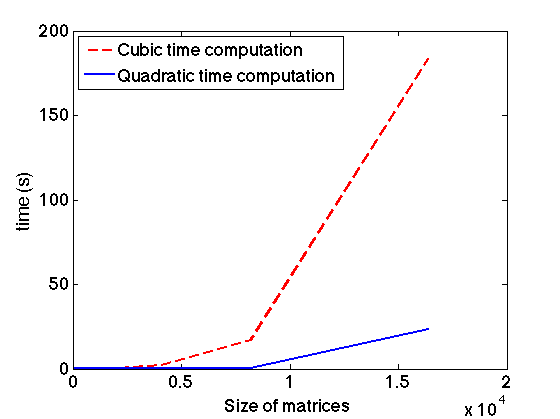
\includegraphics[scale=0.3]{img/ab.png}
\caption{Computation time for $\sum AB$ using standard algorithm vs using inferred optimal algorithm.}
\label{ab}
\end{figure}


Similarly, we found quadratic time computation instead of cubic for similar expressions like : 
\begin{align*}
	\sum ABC\\
	\sum ABCD\\
	\sum AA^T\\
	\sum AA^TA\\
\end{align*}


\subsection{Partition function approximation}

As we shown in Section \ref{partitionfunction}, we can compute $g(x \rightarrow x^k, W)$ for $k = 1, 2$ in
linear time with respect to size of $W$. By use of
our framework, we found rules for $k = 3, 4$. Computation time grows quite fast with power $k$, as we have to consider 
bigger input matrices to cover all possible monomials of particular degree. Table \ref{grammars} shows time necessary to
generate all the rules. It is worth to note, that grammar can be evaluated just once, and the resulting coefficients can 
be stored. Process of partition function approximation involves this steps just once. However, it seems that 
with use of current algorithm we have to stay constrained to powers $k \leq 4$. As we noted in Section \ref{agenda}
it is extremely important and interesting to find pattern how to generate $g(x \rightarrow x^k, W)$ for $k \geq 5$, and
how to generalize optimizations. 

\begin{table}
\tiny
\centering
\begin{tabular}{|l||l|l|}
\hline
Order & Size of grammar & Computation time (s) \\
\hline\hline
2 & 10 & 0.45 \\
3 & 37 & 10.33 \\
4 & & \\
\hline
\end{tabular}
\caption{Table summarizes size and computational time for grammars of specific order.}
\label{grammars}
\end{table}

Resulting equations in non 

\begin{table}
\tiny
\centering
\begin{tabular}{|l||l|l|l|}
\hline
Order & Number of terms & Optimized & Non-optimized \\
& & computation time & computation time  \\
\hline\hline
2 & & & \\
3 & & & \\
4 & & & \\
\hline
\end{tabular}
\caption{Table summarizes computation times of $g(x \rightarrow x^k, W)$.}
\label{grammars}
\end{table}


\section{Computation generalization}\label{agenda}

Presented in this paper method is a brute force over all possible computations, 
which could lead to the target result. It seems to work reasonably well
for polynomials of small degrees $k \leq 4$, however for larger powers 
brute force methods seems to fail. One of major goals of this paper is to
bring a small subset of mathematics, which has tractable brute force automatic proving
system. We look forward to extend this brute force methods to more intelligible approaches, which
could learn based on rules for smaller powers, how to solve problem for larger powers. This would
have two-fold implications in machine learning. Firstly, it would bring machine learning techniques
to the area of automatic theorem proving, which another domain of human intelligence after perception
of vision, or hearing. Secondly, solution to the problem of partition function approximation
could have consequences in unsupervised learning of RBMs, deep Bolzmann machines, and deep
belief networks. 

\section{Conjecture on hardness of partition function approximation}

We present our believes on hardness of approximation of partition function. 
We were not able to prove, or disprove conjectures presented in this chapter.

\begin{conjecture}
Linear combination of terms for a matrix $W$ generated by use of rules :
\begin{itemize}
	\item element wise multiplication
	\item marginalization
	\item repetition
\end{itemize}
consists of $g(x \rightarrow x^k, W)$. Moreover, size of generated grammar
up to degree $k$ is exponential in $k$.
\label{simple}
\end{conjecture}

Corollary and all implications assumes that Conjecture \ref{simple} is valid.

\begin{corollary}
	$g(x \rightarrow k, W)$
	can be computed in exponential time in $k$, but in linear time with respect to size of $W$.
\end{corollary}

\begin{lemma}
	For $x < C$, $e^x$ can be approximated up to $\epsilon$ accuracy in log scale with $\frac{Ce}{\epsilon}$ terms. 
\end{lemma}
\begin{proof}

For every $x < C$ there exists $t < x$, such that :  
\begin{align*}
	e^x = 1 + \frac{x}{1!} + \frac{x^2}{2!} + \dots + \frac{x^{n - 1}}{(n - 1)!} + \frac{x^n}{n!}e^t
\end{align*}
This implies
\begin{align*}
	|e^x - (1 + \frac{x}{1!} + \frac{x^2}{2!} + \dots + \frac{x^{n - 1}}{(n - 1)!}) | < \frac{C^n}{n!}e^C \\
	\sim \exp(n\log{C} + C - n\log{n} + n) < \epsilon
\end{align*}

We require that 
\begin{align*}
	n (1 + \log{C} - \log{n}) < \log{\epsilon} - C \\ 
	n (\log{Ce} - \log{n}) < \log{\epsilon} - C
\end{align*}

Let's assume, that $\log{\epsilon} < -1$, and $1 - Ce < -C$. 
Clearly, this inequality is fulfilled for $n > \frac{Ce}{\epsilon}$ :
\begin{align*}
	\frac{Ce}{\epsilon} (\log{Ce} - \log{\frac{Ce}{\epsilon}}) < \log{\epsilon} - C \\
	\frac{Ce}{\epsilon} \log{\epsilon} < \log{\epsilon} - C\\
	C < \log{\epsilon}(1 - Ce)
\end{align*}


\end{proof}


\section{Summary}
\nocite{*}
\bibliography{bibliography}
\bibliographystyle{icml2012}

\end{document} 

